\section{Simple Harmonic Oscillators: Energy and Damping}
\begin{itemize}
    \item Simple harmonic motion takes place about an equilibrium position and the motion is periodic.
    \item The most simple system is a mass attached to a spring. The restoring force given by Hooke's Law.
          \begin{equation}
              \vec{F} = -k\Delta\vec{x}
          \end{equation}
    \item The period (time/period) and frequency (amount of cycles/second) is related via
          \begin{equation}
              f = \frac{1}{T}
          \end{equation}
          \textit{Note:} This also applies for other oscillatory systems, such as pendulums, LC circuits, i.e.
          \begin{warning}
              Since acceleration is not constant, the standard kinematic equations do not apply.
          \end{warning}
          \begin{example}
              Consider a mass on a spring (and only affected by it). We get a second order differential equation:
              \begin{equation}
                  m\frac{d^2x}{dt^2}=-kx \implies \frac{d^2x}{dt^2}+\frac{k}{m}x = 0.
              \end{equation}
              This is a second order ODE. After solving, we get
              \begin{equation}
                  \omega^2 = \frac{k}{m}.
              \end{equation}
          \end{example}
    \item For a mass on a \textit{vertical spring}, we have a slightly different situation.

          First, note that the equilibrium location shifts. The spring will extend by a distance $\Delta y = (y_1-y_0) = \frac{mg}{k}$, and will then oscillate around this new equilibrium point.

          Let $y_0$ be the equilibrium height (measured from top) and let $y$ be the location of the mass (measured from top). The spring force will then be
          \begin{align}
              \sum F_y = ma & = k(y-y_0)-mg     \\
                            & =k(y-y_0-y_1+y_0) \\
                            & = k(y-y_1)
          \end{align}
          Since $y_1$ is a constant, we can turn the differential equation to be
          \begin{equation}
              \frac{d^2(y-y_1)}{dt^2}=\frac{k}{m}(y-y_1)
          \end{equation}
          and therefore the angular frequency stays the same.
          \begin{warning}
              There are issues related to energy when using this trick. Be careful!
          \end{warning}
    \item The general solution to $\frac{d^2x}{dt^2}+\omega^2 x=0$ is
          \begin{equation}
              x(t) = x_0 + A\cos(\omega t+ \phi_0)
          \end{equation}
          Oftentimes, $x_0=0$ is set as convention. However, the other constants $A$ and $\phi_0$ are determined by initial conditions.
    \item The maximum speed is given by
          \begin{equation}
              v_\text{max} = A\omega
          \end{equation}
          and the maximum acceleration is
          \begin{equation}
              a_\text{max} = A\omega^2
          \end{equation}
          These can be derived by taking the first and second derivatives of $x(t)$.
    \item We can visualize the position, velocity and acceleration graphs:
          \begin{center}
              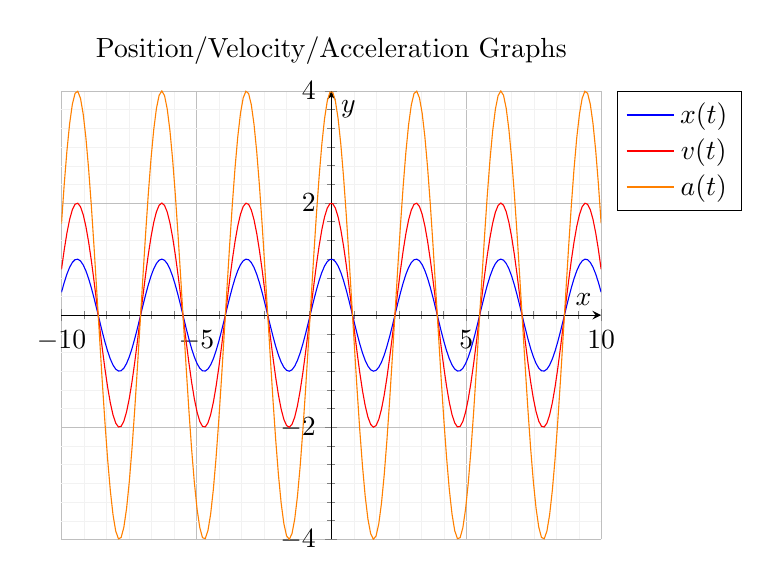
\begin{tikzpicture}
                  \begin{axis}[
                          legend pos=outer north east,
                          title=Position/Velocity/Acceleration Graphs,
                          axis lines = box,
                          xlabel = $x$,
                          ylabel = $y$,
                          variable = t,
                          trig format plots = rad,
                          minor tick num=5, 
                          grid=both,
                          grid style={line width=.1pt, draw=gray!10},
                          major grid style={line width=.2pt,draw=gray!50},
                          axis lines = middle,
                      ]
                      \addplot [
                          domain=-10:10,
                          samples=200,
                          color=blue,
                      ]
                      {cos(2*x)};
                      \addlegendentry{$x(t)$}
                      \addplot [
                          domain=-10:10,
                          samples=200,
                          color=red,
                      ]
                      {2*cos(2*x)};
                      \addlegendentry{$v(t)$}
                      \addplot [
                          domain=-10:10,
                          samples=200,
                          color=orange,
                      ]
                      {4*cos(2*x)};
                      \addlegendentry{$a(t)$};
                  \end{axis}
              \end{tikzpicture}
          \end{center}
    \item There are other ways to express the general solution:
          \begin{equation}
              x(t) = a\cos\omega t + b\sin\omega t
          \end{equation}
          \begin{example}
              Determine the amplitude and phase constant of a pendulum moving with a motion described by a sum of two functions, $x_1(t) = 0.25\cos\omega t$ and $x_2(t) = -0.5\sin\omega t$.
              \vspace{2mm}

              To figure out $\phi_0$, we take the ratio to get
              \begin{equation}
                  \frac{0.5}{0.25}=\tan\phi_0 \implies \tan\phi_0 = 2
              \end{equation}
              Be careful with the assignment of the angle; $\tan(x)$ takes value of $2$ twice during one period, at $x_1=1.107\text{ rad}$ and $x_2=x_1+\pi = 4.25 \text{ rad}$.
              \vspace{2mm}

              To determine which one is correct, you need to look at your original functions: both $\sin\phi_0 > 0$ and $\cos\phi_0 > 0$. Therefore, $\phi_0 = 1.107\text{ rad}$.
          \end{example}
    \item Energy of a simple harmonic oscillator. It has a kinetic energy $K=\frac{1}{2}mv(t)^2$ and potential energy.
    \item The potential energy is related to the restoring force and, by a definition of potential energy, the cahnge in system's potential energy when moving from a position $x_i$ to position $x_f$ is
          \begin{equation}
              \Delta U = - \int_{x_i}^{x_f}(-kx')\dd{x'} = \frac{1}{2}kx_f^2 - \frac{1}{2}kx_i^2.
          \end{equation}
          For a reference, let $x_i=0$ such that we can define $U=\frac{1}{2}kx^2$.
        \item Energy is conserved, i.e.
        \begin{equation}
            U + K = \frac{1}{2}kx^2 + \frac{1}{2}mv^2 = \text{constant}
        \end{equation}
        \item Note that we can show conservation of energy explicitly. The potential energy is
        \begin{equation}
            U = \frac{1}{2}kx^2 = \frac{1}{2}kA^2\cos^2(\omega t)
        \end{equation}
        and the kinetic energy is
        \begin{equation}
            K = \frac{1}{2}mv^2 = \frac{1}{2}m\omega^2A^2\sin^2(\omega t).
        \end{equation}
        Note that $\omega^2 = \frac{k}{m}$ so the total energy is
        \begin{equation}
            E = K + U = \frac{1}{2}kA^2 = \frac{1}{2}m\omega^2
        \end{equation}
        \item When an object is $\frac{1}{\sqrt{2}}A$ from the maximum compression/extension, the kinetic energy equals the potential energy.
        \item \textbf{Physics of small vibrations:} Most systems will oscillate with SHM when the amplitude is small. But what if it's not?
        \begin{example}
            The potential energy of a pendulum is given by
            \begin{equation}
                U = mgy = mgL(1-\cos\theta)
            \end{equation}
            We can use the Taylor series:
            \begin{equation}
                f(x) = f(a) + \frac{x-a}{1!}\left(\frac{\partial f}{\partial x}\right)_{x=a} + \frac{(x-a)^2}{2!}\left(\frac{\partial^2 f}{\partial x^2}\right)_{x=a} + \cdots
            \end{equation}
            The energy about $x=0$ is then:
            \begin{equation}
                U(x) = U(0) + x\frac{dU}{dx}\bigg\vert_{x=0} + \frac{x^2}{2}\frac{d^2U}{dt^2}\bigg\vert_{x=0} + \cdots.
            \end{equation}
            Using this, we can make the lowest order (nonzero) approximation to be 
            \begin{equation}
                U = \frac{1}{2}mgL \theta^2
            \end{equation} 
        \end{example}
        \item In this course, any angle smaller than $10^\circ$ would be considered a \textit{small angle.}
        \item For example, the differential equation that describes a pendulum is 
        \begin{equation}
            L\frac{d^2\theta}{dt^2}=-g\sin\theta
        \end{equation}
        If $\theta \ll 1$, then we can approximate $\theta \approx \sin\theta$ such that the differential equation becomes 
        \begin{equation}
            \frac{d^2\theta}{dt^2} = -\frac{g}{L}\theta
        \end{equation}
        which is the familiar second order differential equation. The period is:
        \begin{equation}
            T = \frac{2\pi}{\omega} = 2\pi \sqrt{\frac{L}{g}}.
        \end{equation}
        \item The energy of a pendulum is given by
        \begin{equation}
            E = K + U = \frac{1}{2}mv^2 + mg\left(\frac{x^2}{2L}\right).
        \end{equation}
\end{itemize}